\chapter{Modello Analitico}
Dal modello simulativo è stato possibile ricavare il tasso di arrivo di richeste HTTP, dato fondamentale per poter eseguire un modello analitico. Dalla configurazione standard si è ricavato il valore: 
\begin{equation}
\lambda =  3308.79 \frac{richieste}{sec}
\end{equation}
Le probabilità di arrivo di richieste di classe r, sono date dalla formula:
\begin{equation}
p_{r} = \frac{count_{r}}{observation}
\end{equation}
\begin{flushleft}
Di seguito si riportano nuovamente i valori già presentati nel capitolo 2
\end{flushleft}
\begin{table}[H]
\begin{center}
\begin{tabular}{||c|c|c||}
\hline
Classe	&Dimensione(byte)		&Richieste \\ 
\hline\hline
1 &10281 &9999995\\ \hline
2 &279513744 &4 \\ \hline
3 &715827882 &1 \\ \hline
\end{tabular}
\end{center}
\caption{Risultati clustering}
\label{risclustering}
\end{table}
\begin{table}[H]
\begin{center}
\begin{tabular}{||c|c||}
\hline
Classe		&Prob. arrivo richieste classe R	\\
\hline
\hline
1		&0.9999995	\\
\hline
2		&0.0000004\\
\hline
3		&0.0000001\\
\hline
\end{tabular}
\end{center}
\caption{Probabilita' di arrivo delle richieste}
\label{test_2}
\end{table}
\begin{flushleft}
Il tasso di richieste per la singola classe è dato dalla formula:
\end{flushleft}
\begin{equation}
\lambda_{r} = \lambda*p_{r}
\end{equation}
Utilizzazione:
\begin{equation}
U_{i,r}(\overrightarrow{\lambda}) = \lambda_{r} * D_{i,r}
\end{equation}
\begin{equation}
U_{i}(\overrightarrow{\lambda})  = \sum_{r=1}^{K} U_{i,r}(\overrightarrow{\lambda})
\end{equation}
Lunghezza coda:
\begin{equation}
n_{i,r}(\overrightarrow{\lambda}) = \frac{U_{i,r}(\overrightarrow{\lambda})}{1 - U_{i}(\overrightarrow{\lambda})}
\end{equation}
\begin{equation}
n_{i}(\overrightarrow{\lambda}) = \sum_{r=1}^{K} n_{i,r}(\overrightarrow{\lambda})
\end{equation}
Tempo di residenza:
\begin{equation}
R_{i,r}(\overrightarrow{\lambda}) = \frac{D_{i,r}}{1 - U_{i}(\overrightarrow{\lambda})}
\end{equation}\\
Per $D_{i,r}$ si intende la domanda di servizio della risorsa i-esima per richieste di classe r-esima. Per quanto concerne le domande di servizio, queste sono le stesse presentate nel modello simulativo, con la differenza che in questo caso, quando è necessario fornire la dimensione del documento, per la classe r bisogna usare il centroide r-esimo. I risultati ottenuti per le componenti del web server dovranno poi essere opportunamente mediati per il numero di server (nel caso delle schede di rete e delle CPU) e per il numero di server moltiplicato per il numero di dischi (nel caso dei dischi dei web server). Questa assunzione è valida nel caso il carico sia equamente ripartito tra i server e i dischi.
\section{Presentazione dei risultati}
Si presentano di seguito i risultati ottenuti applicando il modello analitico, sia alla rete in configurazione standard che nelle sue varianti.
\subsection{Risultati standard}
\begin{table}[H]
\begin{center}
\begin{tabular}{||c|c|c|c|c||}
\hline
Centro &Classe1 &Classe2 &Classe3 &Totale\\
\hline
\hline
 cpu web server i-esimo: 	&0.6684421	&0.0000003	&0.0000001	&0.6684424	\\\hline
 disco i-esimo: 	&0.3230367	&0.0029392	&0.0018818	&0.3278577	\\\hline
 inLink: 	&0.3070557	&0.0000001	&0.0000000	&0.3070559	\\\hline
 outLink: 	&0.2874940	&0.0030771	&0.0019701	&0.2925412	\\\hline
 cpu web switch: 	&0.6893309	&0.0000003	&0.0000001	&0.6893313	\\\hline
 LAN: 	&0.2867530	&0.0030050	&0.0019239	&0.2916819	\\\hline
 LS1: 	&0.3013115	&0.0030771	&0.0019701	&0.3063587	\\\hline
 LS2:	&0.2867530	&0.0030050	&0.0019239	&0.2916819	\\\hline
 LW2: 	&0.0043447	&0.0000455	&0.0000292	&0.0044194	\\\hline
\end{tabular}
\end{center}
\caption{Utilizzazioni}
\label{utilizzazioni}
\end{table}
Dalla tabella presentata si può notare che, anche attraverso la risoluzione analitica, i vincoli sulle utilizzazioni sono rispettati e che sono molto simili a quelli presentati nel modello simulativo, se si escludono una differenza di circa il 3\% per quanto riguarda l'utilizzazione dei dischi.
\begin{figure}[H]
\begin{center}
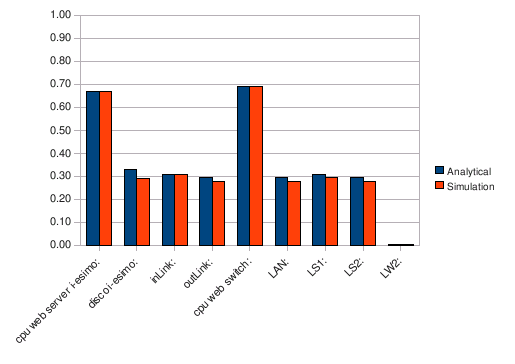
\includegraphics[scale=0.8]{etc/utilizzazione_standard.png}
\caption{Confronto utilizzazioni analitico-simulativo}
\label{confronto}
\end{center}
\end{figure}
\begin{table}[H]
\begin{center}
\begin{tabular}{||c|c|c|c|c||}
\hline
Centro &Classe1 &Classe2 &Classe3 &Totale\\
\hline
\hline
 cpu web server i-esimo: 	&2.0160664	&0.0000008	&0.0000002	&2.0160674	\\\hline
 disco i-esimo: 	&0.4806076	&0.0043730	&0.0027997	&0.4877803	\\\hline
 inLink: 	&0.4431176	&0.0000002	&0.0000000	&0.4431178	\\\hline
 outLink: 	&0.4063756	&0.0043495	&0.0027847	&0.4135099	\\\hline
 cpu web switch: 	&2.2188614	&0.0000009	&0.0000002	&2.2188625	\\\hline
 LAN: 	&0.4048366	&0.0042424	&0.0027162	&0.4117952	\\\hline
 LS1: 	&0.4343910	&0.0044362	&0.0028402	&0.4416674	\\\hline
 LS2: 	&0.4048366	&0.0042424	&0.0027162	&0.4117952	\\\hline
 LW2: 	&0.0043640	&0.0000457	&0.0000293	&0.0044390	\\\hline
\end{tabular}
\end{center}
\caption{Lunghezza Code}
\label{lunghezzacode}
\end{table}
Come era logico aspettarsi, data la natura della formula che rappresenta la lunghezza della coda, le risorse più utilizzate sono quelle che presentano i valori più alti.
\begin{table}[H]
\begin{center}
\begin{tabular}{||c|c|c|c||}
\hline
Centro &Classe1 &Classe2 &Classe3\\
\hline
\hline
 cpu web server i-esimo: 	&0.0402142	&0.0402142	&0.0402142	\\\hline
 disco i-esimo: 	&0.1150395	&2616.8025427	&6701.5469112	\\\hline
 inLink: 	&0.0001339	&0.0001339	&0.0001339	\\\hline
 outlink: 	&0.0001228	&3.2863295	&8.4162080	\\\hline
 cpu web switch: 	&0.0006706	&0.0006706	&0.0006706	\\\hline
 LAN: 	&0.0001185	&3.2054117	&8.2089814	\\\hline
 LS1: 	&0.0001313	&3.3518001	&8.5838670	\\\hline
 LS2: 	&0.0001185	&3.2054117	&8.2089814	\\\hline
 LW2: 	&0.0000843	&2.2805296	&5.8403809	\\\hline
\end{tabular}
\end{center}
\caption{Tempo di residenza}
\label{tempodiresidenza}
\end{table}
In questa tabella si notano immediatamente i valori spropositati dei tempi di residenza dei dischi del web server nel caso di richieste di Classe 2 e 3. Questi valori sono dovuti al fatto che i file appartenenti a queste due classi sono dell'ordine di centinaia di megabyte e dunque le operazioni di lettura dal disco richiedono svariati minuti per essere completate (si ricorda al lettore che i centroidi di classe 2 e 3 hanno una dimensione rispettivamente di 279 MB e 715 MB).

\subsection{Risultati proxy}
\begin{table}[H]
\begin{center}
\begin{tabular}{||c|c|c|c|c||}
\hline
Centro &Classe1 &Classe2 &Classe3 &Totale\\
\hline
\hline
 cpu web server i-esimo: 	&0.4010653	&0.0000002	&0.0000000	&0.4010655	\\\hline
 disco i-esimo: 	&0.1938220	&0.0017635	&0.0011291	&0.1967146	\\\hline
 inLink: 	&0.1842334	&0.0000001	&0.0000000	&0.1842335	\\\hline
 outLink: 	&0.1724964	&0.0018463	&0.0011821	&0.1755247	\\\hline
 cpu web switch: 	&0.4135985	&0.0000002	&0.0000000	&0.4135987	\\\hline
 LAN: 	&0.1720518	&0.0018030	&0.0011544	&0.1750092	\\\hline
 LS1: 	&0.1807869	&0.0018463	&0.0011821	&0.1838152	\\\hline
 LS2:	&0.1720518	&0.0018030	&0.0011544	&0.1750092	\\\hline
 LW2: 	&0.0026068	&0.0000273	&0.0000175	&0.0026517	\\\hline
\end{tabular}
\end{center}
\caption{Utilizzazioni}
\label{utilizzazioni}
\end{table}
Le utilizzazioni, nel caso dell'introduzione del proxy server, tendono a diminuire notevolmente, in modo particolare se si considerano le CPU del Web Switch e dei Web Server. Anche in questo caso, i risultati sono molto simili a quelli ottenuti col modello simulativo.
\begin{figure}[H]
\begin{center}
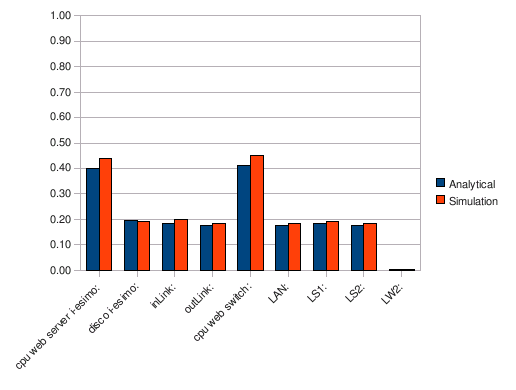
\includegraphics[scale=0.8]{etc/utilizzazione_proxy.png}
\caption{Confronto utilizzazioni analitico-simulativo con proxy}
\label{Confronto proxy}
\end{center}
\end{figure}
\begin{table}[H]
\begin{center}
\begin{tabular}{||c|c|c|c|c||}
\hline
Centro &Classe1 &Classe2 &Classe3 &Totale\\
\hline
\hline
 cpu web server i-esimo: 	&0.6696312	&0.0000003	&0.0000001	&0.6696315	\\\hline
 disco i-esimo: 	&0.2412866	&0.0021954	&0.0014056	&0.2448876	\\\hline
 inLink: 	&0.2258409	&0.0000001	&0.0000000	&0.2258410	\\\hline
 outLink: 	&0.2092196	&0.0022393	&0.0014337	&0.2128926	\\\hline
 cpu web switch: 	&0.7053166	&0.0000003	&0.0000001	&0.7053170	\\\hline
 LAN: 	&0.2085500	&0.0021855	&0.0013992	&0.2121347	\\\hline
 LS1: 	&0.2215024	&0.0022621	&0.0014483	&0.2252128	\\\hline
 LS2: 	&0.2085500	&0.0021855	&0.0013992	&0.2121347	\\\hline
 LW2: 	&0.0026138	&0.0000274	&0.0000175	&0.0026587	\\\hline
\end{tabular}
\end{center}
\caption{Lunghezza Code}
\label{lunghezzacode}
\end{table}
L'introduzione del proxy comporta anche un minore accodamento delle richieste. Si può notare infatti come ogni centro presenti delle code inferiori ad uno.
\begin{table}[H]
\begin{center}
\begin{tabular}{||c|c|c|c||}
\hline
Centro &Classe1 &Classe2 &Classe3\\
\hline
\hline
 cpu web server i-esimo: 	&0.0222618	&0.0222618	&0.0222618	\\\hline
 disco i-esimo: 	&0.0962583	&2189.5874861	&5607.4629303	\\\hline
 inLink: 	&0.0001138	&0.0001138	&0.0001138	\\\hline
 outlink: 	&0.0001054	&2.8199060	&7.2217088	\\\hline
 cpu web switch: 	&0.0003553	&0.0003553	&0.0003553	\\\hline
 LAN: 	&0.0001018	&2.7520924	&7.0480417	\\\hline
 LS1: 	&0.0001116	&2.8485547	&7.2950694	\\\hline
 LS2: 	&0.0001018	&2.7520924	&7.0480417	\\\hline
 LW2: 	&0.0000842	&2.2764875	&5.8300290	\\\hline
\end{tabular}
\end{center}
\caption{Tempo di residenza}
\label{tempodiresidenza}
\end{table}
L'introduzione del proxy server non risolve completamente il problema della gestione di file di Classe 2 e 3 all'interno dei dischi, ma permette comunque di ottenere un miglioramento non trascurabile.  
\subsection{Risultati Link Addizionale}
\begin{table}[H]
\begin{center}
\begin{tabular}{||c|c|c|c|c||}
\hline
Centro &Classe1 &Classe2 &Classe3 &Totale\\
\hline
\hline
 cpu web server i-esimo: 	&0.6684421	&0.0000003	&0.0000001	&0.6684424	\\\hline
 disco i-esimo: 	&0.3230367	&0.0029392	&0.0018818	&0.3278577	\\\hline
 inLink: 	&0.3070557	&0.0000001	&0.0000000	&0.3070559	\\\hline
 outLink: 	&0.2874940	&0.0030771	&0.0019701	&0.0000000	\\\hline
 cpu web switch: 	&0.3446655	&0.0000001	&0.0000000	&0.3446656	\\\hline
 LAN: 	&0.0089958	&0.0000000	&0.0000000	&0.0089958	\\\hline
 LS1: 	&0.0138175	&0.0000000	&0.0000000	&0.0138175	\\\hline
 LS2:	&0.0089958	&0.0000000	&0.0000000	&0.0089958	\\\hline
 LW2: 	&0.0001363	&0.0000000	&0.0000000	&0.0001363	\\\hline
 LINK\_ADD: 	&0.4622090	&0.0049471	&0.0031674	&0.4703235	\\\hline
 LW3: 	&0.0070032	&0.0000750	&0.0000480	&0.0071261	\\\hline
\end{tabular}
\end{center}
\caption{Utilizzazioni}
\label{utilizzazioni}
\end{table}
Come già evidenziato nel modello simulativo, l'introduzione del link addizionale permette di ridurre notevolmente le utilizzazioni del web switch e delle componenti di rete “interne” (LS1, LS2, L2, LW2). In questo caso la risorsa collo di bottiglia diventa la CPU del Web Server. Anche in quest'ultimo caso, le differenze rispetto alle utilizzazioni  ottenuti col modello simulativo sono minime.
\begin{figure}[H]
\begin{center}
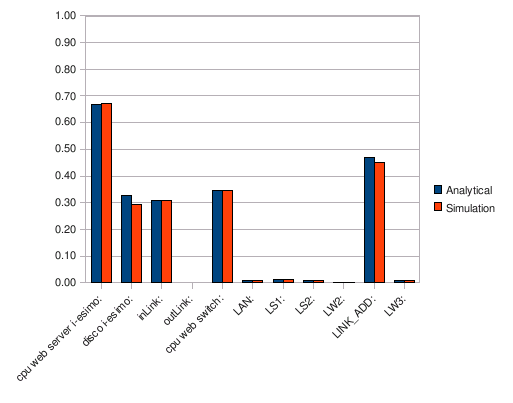
\includegraphics[scale=0.8]{etc/utilizzazione_link_add.png}
\caption{Confronto utilizzazioni analitico-simulativo con link addizionale}
\label{confronto link add}
\end{center}
\end{figure}
\begin{table}[H]
\begin{center}
\begin{tabular}{||c|c|c|c|c||}
\hline
Centro &Classe1 &Classe2 &Classe3 &Totale\\
\hline
\hline
 cpu web server i-esimo: 	&2.0160664	&0.0000008	&0.0000002	&2.0160674	\\\hline
 disco i-esimo: 	&0.4806076	&0.0043730	&0.0027997	&0.4877803	\\\hline
 inLink: 	&0.4431176	&0.0000002	&0.0000000	&0.4431178	\\\hline
 outLink: 	&0.4063756	&0.0043495	&0.0027847	&0.0000000	\\\hline
 cpu web switch: 	&0.5259383	&0.0000002	&0.0000001	&0.5259386	\\\hline
 LAN: 	&0.0090774	&0.0000000	&0.0000000	&0.0090774	\\\hline
 LS1: 	&0.0140111	&0.0000000	&0.0000000	&0.0140111	\\\hline
 LS2: 	&0.0090774	&0.0000000	&0.0000000	&0.0090774	\\\hline
 LW2: 	&0.0001363	&0.0000000	&0.0000000	&0.0001363	\\\hline
 LINK\_ADD: 	&0.8726251	&0.0093399	&0.0059798	&0.8879447	\\\hline
 LW3: 	&0.0070534	&0.0000755	&0.0000483	&0.0071773	\\\hline
\end{tabular}
\end{center}
\caption{Lunghezza Code}
\label{lunghezzacode}
\end{table}
Le code risultano essere tutte minori di uno, ad eccezione della CPU del Web Server che presenta un valore pari a 2 a causa dell'alta utilizzazione.
\begin{table}[H]
\begin{center}
\begin{tabular}{||c|c|c|c||}
\hline
Centro &Classe1 &Classe2 &Classe3\\
\hline
\hline
 cpu web server i-esimo: 	&0.0402142	&0.0402142	&0.0402142	\\\hline
 disco i-esimo: 	&0.1150395	&2616.8025427	&6701.5469112	\\\hline
 inLink: 	&0.0001339	&0.0001339	&0.0001339	\\\hline
 outlink: 	&0.0001228	&3.2863295	&8.4162080	\\\hline
 cpu web switch: 	&0.0001590	&0.0001590	&0.0001590	\\\hline
 LAN: 	&0.0000027	&0.0000027	&0.0000027	\\\hline
 LS1: 	&0.0000042	&0.0000042	&0.0000042	\\\hline
 LS2: 	&0.0000027	&0.0000027	&0.0000027	\\\hline
 LW2: 	&0.0000027	&0.0000027	&0.0000027	\\\hline
 LINK\_ADD: 	&0.0002637	&7.0568543	&18.0724278	\\\hline
 LW3: 	&0.0001407	&3.7646776	&9.6412454	\\\hline\hline
\end{tabular}
\end{center}
\caption{Tempo di residenza}
\label{tempodiresidenza}
\end{table}
Le considerazioni fatte sui tempi di residenza nel caso standard sono valide anche con l'introduzione del link addizionale. 
